\documentclass[a4paper,12pt]{article}

\usepackage{epsfig}

\setlength{\oddsidemargin}{0in}
\setlength{\textwidth}{6.5in}

\setlength{\topmargin}{-0.25in}
\setlength{\textheight}{10.5in}

\begin{document}

\newcommand{\thisproj}{\bf GUI To Catalog Description}

\makeatletter                       % Make '@' accessible.
\pagestyle{myheadings}              % We do our own page headers.
\def\@oddhead{\bf Aurora - \thisproj \hfill (rly)} 
\hbadness=10000                     % No "underfull hbox" messages.
\makeatother     

\section*{Assumptions}
This document assumes knowledge of reading the catalogs produced by an older version of the GUI.  More specifically, the older version had no support for superboxes, but was able to load and process join and filter boxes, in addition to the source stream nodes (from the beginning) and the application nodes (at the end).

Furthermore, the database table definition items are listed in the order that they are saved into the database by the GUI.

\section*{Database table definitions}

\hspace{.5in}
\textbf{ArcRecordDbt}
\vspace{.1in}

\begin{tabular}{|l|l|l|}
\hline
\em type & \em name    & \em notes \\\hline
int       & id            & unique arc id \\
float     & rate          &               \\
int       & schemaId      &               \\
int       & sourceNodeId  & unique box id the source node \\
int       & destinationNodeId & unique box id of the destination node \\
int       & sourcePortId  & index of the port the arc is connected to \\
int       & destinationPortId & index of the port the arc is connected to \\
int       & cpFlag        &                \\
int       & parentId      & unique box id of the superbox containing this arc \\\hline        
\end{tabular}

\vspace{.1in}
\hspace{.5in}
\textbf{BoxRecordDbt}
\vspace{.1in}

\begin{tabular}{|l|l|l|}
\hline
\em type & \em name    & \em notes \\\hline
int       & id            & unique arc id \\
int       & typeId        &               \\
          & \vdots        &               \\
String    & label         & saved in UTF encoding \\
int       & parentId      & unique box id of the superbox containing this box \\\hline
\end{tabular}

\vspace{.1in}
\hspace{.5in}
\textbf{Definitions}
\vspace{.1in}

\begin{tabular}{|l|c|}
\hline
\em box type & \em enumerated value \\\hline
filter         & 0 \\
map            & 1 \\
windowed map   & 2 \\
merge          & 3 \\
resample       & 4 \\
join           & 5 \\
drop           & 6 \\
inputportnode  & 7 \\
outputportnode & 8 \\\hline           
\end{tabular}


\newpage

\section*{Usage and Description}

With the addition of superbox support in the GUI, the only changes in the catalog that require notice are the sourcePortId and destinationPortId values from ArcRecordDbt, and the InputPortNode and OutputPortNode enumeration definitions.

One previous capability not supported in the earlier version was box labels.  BodRecords now store a string in UTF encoding that is defined by the user.

See the below diagram for a clear illustration on how to connect two boxes through a superbox.  Below, we have two boxes \textit{a} and \textit{c} that, while connected, are separated by superbox \textit{b}.  All of the items, box \textit{a}, superbox \textit{b}, box \textit{c}, port node \textit{d}, and arcs \textit{e} and \textit{f} will have records in the tables that are defined in their respected table definitions in the previous page.

Note that the port node \textit{d} by ether an enumerated value of 7 or 8, depending on whether it is an input port node or an output port node.

\begin{figure}[ht]
\includegraphics[scale=.8]{gui2catalog.ps}
\end{figure}

In order to semantically connect a source node inside a superbox to a targetnode outside of the superbox, the all that is required is to switch the ``sources'' with the ``destinations'' for the node id.

\end{document}
